
\graphicspath{ {mainmatter/Ouzounian_2012/} }

\title*{2012: To be inside someone else's dream: Music for Sleeping \& Waking Minds}
\titlerunning{Music for Sleeping \& Waking Minds}


\author{Gascia Ouzounian, R. Benjamin Knapp, Eric Lyon and R. Luke DuBois}
\authorrunning{Ouzounian et al.}


% \institute{Gascia Ouzounian \at Sonic Arts Res. Centre, Queen's University, Belfast, Northern Ireland BT7 1NN, \email{g.ouzounian@qub.ac.uk}
% \and R. Benjamin Knapp \at Inst. for Creativity, Arts, and Technology, Virginia Tech University, Blacksburg, VA, 24060, \email{benknapp@vt.edu}
% \and Eric Lyon \at School of Performing Arts $\vert{}$ Music, Virginia Tech, Blacksburg, VA 24061 Original affiliation for Eric Lyon:
% Eric Lyon, Sonic Arts Research Centre, Queen's University Belfast, Northern Ireland BT7 1NN \email{ericlyon@vt.edu},
%  \and R. Luke DuBois \at Brooklyn Experimental Media Center, Polytechnic Inst. of NYU, Brooklyn, NY 11201 \email{rdubois@poly.edu}}
%
%
\maketitle

\abstract*{\textit{Music for Sleeping \& Waking Minds} (2011-2012) is a new, overnight work in which four performers fall asleep while wearing custom designed EEG sensors which monitor their brainwave activity. The data gathered from the EEG sensors is applied in real time to different audio and image signal processing functions, resulting in continuously evolving multi-channel sound environment and visual projection. This material serves as an audiovisual description of the individual and collective neurophysiological state of the ensemble. Audiences are invited to experience the work in different states of attention: while alert and asleep, resting and awakening.}

\section{Introduction}

In her discussion of Bill Viola's \textit{Sleep of Reason} (1988)---an installation that intersperses long segments of video of a sleeping man's head with brief interludes of nightmarish images and loud noises---the cultural theorist and critic Mieke Bal asks: `To be inside someone else's dream: could that not be a definition of the experience of art'? \cite{Bal:2006} Indeed, much of the art of the last century (in particular) can be seen as belonging to the repository of dreams: a record of dreaming, a meditation on the dream, an ode to the dreamer. (See Gamwell 2000). \cite{Gamwell:2000}

This art is often representational, conveying dream imagery or images of sleep.
Andy Warhol's first film, \textit{Sleep} (1963), a five-hour film of the poet
John Giorno sleeping, is a celebrated example. Other works do not necessarily
represent sleep or sleep states, but are instead posited as productions of the
`subconscious' or `unconscious' mind: works that result, for example, from the
use of chance methods, or the automatistic methods favored by Surrealists and
Dadaists. In other cases, sleeping itself is performed for an audience. In his
\textit{Dream Event }(3-5 December 1971), the Fluxus artist Geoffrey Hendricks
fasted, slept, and kept a log of his thoughts for forty-eight hours in a
Manhattan gallery.  For her work \textit{Slumber }(1993), the Bahamian artist
Janine Antoni slept in the Guggenheim Museum in New York City for several weeks.
An electroencephalograph (EEG) machine recorded Antoni's brainwaves, producing
patterns that she subsequently wove into the blanket under which she slept. In
more rare examples, audiences themselves have been invited to sleep as part of an
artwork.  From 25 October 2008 to 6 January 2009, the Guggenheim accepted
overnight reservations for Carsten H\"{o}ller's \textit{Revolving Hotel Room}, an
installation in which the interior of a hotel suite was mounted on a rotating
platform inside the museum.  Participants in \textit{Revolving Hotel Room }could,
ostensibly, have their own private sleepover at the Guggenheim.

\textit{Music for Sleeping \& Waking Minds }(\textit{MS\&WM}) is a new work that
belongs to, and in some ways diverges from, this rich lineage of sleep and
dream-based art. Composed and conceived by Gascia Ouzounian, and featuring
physiological interface and interaction design and audio/video behaviors by R.
Benjamin Knapp, audio interface and interaction design by Eric Lyon, and visual
interface and interaction design by R. Luke DuBois, \textit{MS\&WM }invites
audiences and performers alike to fall asleep and awaken to sounds that are
generated by the brainwave activity of four `performers.' During the course of
one night, the four individuals fall asleep and awaken as they naturally would. 
As they do, their brainwaves generate and process sound and image. This sound
emerges as a continuously evolving, dense electronic drone made up of multiple
tones whose aural characteristics (timbre, spatial location, frequency, duration,
amplitude, etc.) evolve in simple and minute ways according to changes in
brainwave activity. The sound environment is projected over eight loudspeakers
that surround the audience. The visual projection, which is similarly derived
from EEG signals, follows a parallel process in light and colour. Audiences, who
are invited to bring anything that they need to ensure comfortable sleep, can
experience the work in different states of attention including sleeping and
awakening.

In translating the brainwave activity of four sleeping performers into an
immersive audiovisual environment, \textit{Music for Sleeping \& Waking Minds
}literally invites listeners to be inside someone else's dream: a collective
dream that is at once performed, represented, and produced in and between
multiple states of consciousness, and articulated in sound and light.

\section{Compositional Elements}

\textit{MS\&WM} can be thought of as an audiovisual description of the
individual and collective neurophysiological states of four individuals. It is
perhaps unique in the NIME community in that the performers' only task is to
sleep and awaken while wearing EEG sensors. The data gleaned from the EEG sensors
is transmitted to computers that show a visual representation of each performer's
brainwave activity (in the EyesWeb software environment), and apply these
brainwave signals in real time to different audio and image signal processing
functions (in Max/MSP and Jitter).

In the first presentations of \textit{MS\&WM}, which took place in the summer of
2011, the synthesized sound comprised a set of sixteen sine tones that were
modulated by the ensemble's brainwave activity.  Each performer was assigned four
tones at the outset of the event, and each performer was brought into the mix in
turn (at around 10 minute intervals), such that his or her contribution to the
overall mix could potentially be identifiable. The thought was that these
staggered entrances would allow listeners to observe the ways in which each
performer contributes to the emerging `collective consciousness' being described
in sound.  This emergent consciousness---one that could be heard simultaneously
within multiple states of attention---was neither predictable nor controlled. 
It evolved as a kind of dialogue between minds, a dialogue that was
simultaneously `conscious' and not.

As an artwork, \textit{MS\&WM} is principally concerned with perception and
communication, specifically as these emerge within and between different states
of attention: How does our perception of sound and light change between different
states of attention, and how is this shift experienced (physiologically,
emotionally, etc.)? How do we communicate these experiences, and what are the
terms of our communications?

The decision to base the composition of \textit{MS\&WM }on a rich, mostly
static, synthesized drone emerged for a number of reasons.  In the first
instance, the work was conceived as the second in a series of overnight
compositions. In the first of these, \textit{EDEN EDEN EDEN} (2009), an
audiovisual work by Gascia Ouzounian and filmmaker Chlo\'e Griffin, an ensemble of
fourteen string players builds and deconstructs a harmonic series over the course
of about six hours, continuously tuning and detuning this rich chord according to
a predetermined process.  In using a continuously evolving drone as the basic
musical material of both compositions, the idea was to allow listeners to project
their own perceived structure upon the work rather than experience it according
to predefined structures. In contrast to fragmented musical forms, the drone also
serves as a more flexible accompaniment to the listener's imagination and
thoughts (or sequences of thoughts), which may be of any duration, and which
might emerge or fade at any stage.

In this sense, \textit{MS\&WM }is more closely aligned with works that `invite
the dreamer to dream' rather than depict or define particular dreams---as in the
Finnish artist Maaria Wirkkala's \textit{Dream Screen}, for example, which
consisted of a large black rectangle on the surface of a gallery wall. `By
transforming the blackness into a surface on which to view oneiric projections in
the night, [Wirkkala] presented [\textit{Dream Screen}] as not a physical,
``literal'' surface but as an expanse filled with meaning' \cite[p.31]{Gamwell:2000}. It owes a particular debt to La Monte Young's conception of continuous
periodic, composite waveform environments; his idea of a `drone state of mind';
and Young and Marian Zazeela's \textit{Dream House}, `a time installation
measured by a setting of continuous frequencies in sound and light' currently in
its nineteenth year of exhibition in lower Manhattan (see Young and Zazeela) \cite{Young:2012}.

The drone basis of \textit{MS\&WM }also allowed for changes in individual
performers' brainwave activity to be articulated in perceptible ways, while at
the same time providing a continuous field of sound that would ideally promote,
rather than disrupt, sleep among participants and audiences.

\begin{figure}[t]
\centering
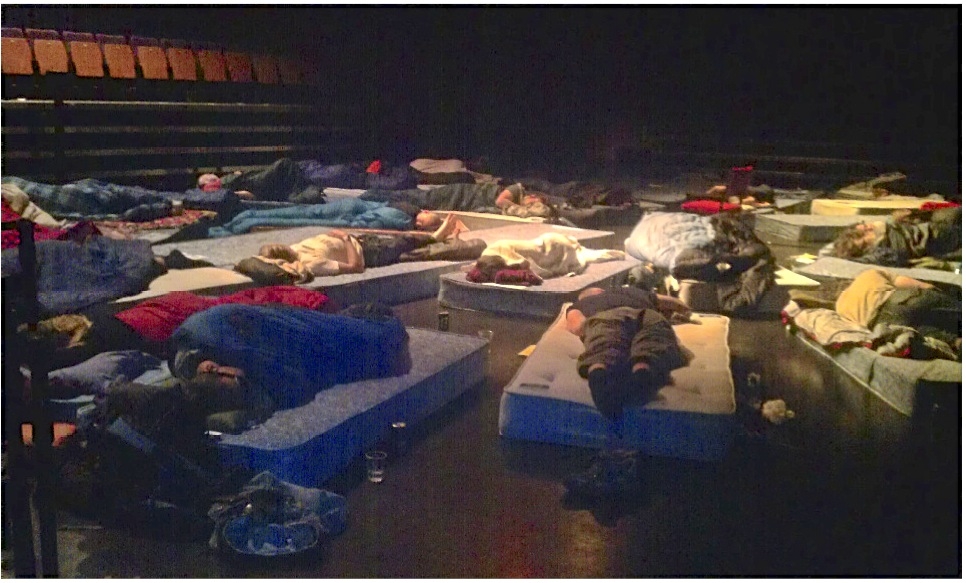
\includegraphics[width=\textwidth]{img-1.jpg}
\caption{Audiences at the premiere of \emph{Music for Sleeping and Waking Minds}. BEAM Festival, Uxbridge 25-26 June 2011. Photograph by Gascia Ouzounian.}
\end{figure}

\section{Mapping Sleep to Sound}

\subsection{Background}

Techniques for deriving states of consciousness during sleep by measuring brainwave activity began over a half century ago \cite{Loomis:1937}. Using an array of electrodes across the scalp, Loomis measured the change in electrical activity using the electroencephalogram (EEG) during sleep and determined that there were specific patterns that repeated themselves over the course of the night.  Since then, these patterns have become known as the five stages of sleep: stages 1-4 and Rapid Eye Movement (REM) sleep \cite{Dement:1957}. Sleep stage 1 corresponds to when the eyes are closed and the individual is drowsy. It is identified by the presence of 8-12Hz waves (alpha waves) within the EEG. Sleep stage 2 is the predominant sleep stage during the night and is noted by the diminishment of the alpha waves as well as the appearance of random signal bursts in the region of 12-16Hz known as sleep spindles (and associated k-complexes). Stage three begins the appearance of slow waves around 4-8Hz known as delta waves.  Stage 4 sleep is known as `deep sleep' and is only differentiated from stage three by the quantity of the delta wave activity. REM sleep, often (although not exclusively) associated with dreaming, is noted by bursts in the EEG caused by the eyes darting back and forth (EOG).

Over the course of a night, roughly every ninety minutes, a normal sleeper will
cycle through these stages.  As the night progresses, the typical sleeper will
experience less and less deep (stage 4) sleep and will move back and forth
between the other stages in a less sequential pattern, even waking up from time
to time. (For a good overview of sleep staging and the EEG see Carskadon and
Rechtschaffen, 2005) \cite{Carskadon:2005}.

\subsection{The Hardware Configuration}

As previously mentioned, \textit{MS\&WM} has four `performers' whose brainwaves drive the 8-channel audio element of the piece. As seen in Figure~\ref{Ouzounian:fig:1} below, each performer wears a single headband from Infusion Systems\footnote{\url{http://infusionsystems.com}} that contains three dry electrodes placed on the forehead for measuring the frontal lobe EEG. This placement also enables the electrodes to pick up the EOG associated with REM sleep.  Inside the band is also a bi-axial accelerometer for measuring motion of the head.  The band and the accelerometer are connected to a Bluetooth radio to transmit the data to a PC running EyesWeb software that, in real-time, combines the data streams from all four performers, extracts the relevant features of the EEG and the motion signals and then send the data to a second PC running Max/MSP to map these features into sound.



\begin{figure}[t]
\centering
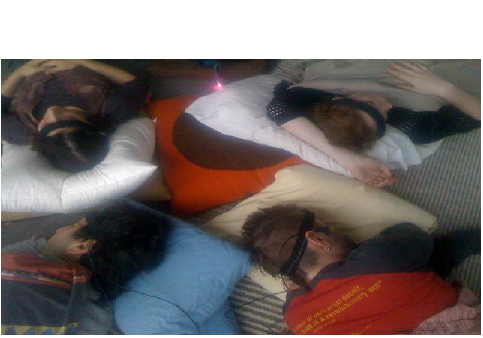
\includegraphics[width=\textwidth]{img-2-eps-converted-to-crop.pdf}
\caption{Four performers wearing headbands containing EEG dry electrodes and 2D accelerometers.  Diapason Gallery, New York City, 4-5 June 2011. Photograph by Gascia Ouzounian.}
\label{Ouzounian:fig:1}
\end{figure}

\subsection{The Mapping Software}

As shown in Figure~\ref{Ouzounian:fig:2}, the auditory representation of the sleep stages
of the performers relies on continuous mappings of the EEG and accelerometer
signals to parameters of a continuously evolving, 8-channel sound environment. 
The\textit{ }sound consists of sixteen tones of variable spectrum.  Each
performer influences four of these tones.  As a performer enter sleep stage 1,
the presence of alpha waves applies tremolo to the four tones assigned to that
performer.  As the performer slowly transitions to sleep stage 2, the tremolos
decrease.  At the same time, the beginning presence of sleep spindles triggers
enveloped tones processed by delays with feedback.  As the performer moves into
stage 3 sleep, the presence of slow wave (Delta) activity reduces the timbral
complexity of each of the tones.  When the performer finally reaches stage 4
(deep) sleep, the complexity is at its minimum.  Also, each time a performer
reaches this stage, one sine tone is removed from the four tones.  This means
that if the performer achieves deep sleep three or more times in a night, only
one tone will be present at the end.  This enables listeners to not only
experience the changing sound environment within one sleep cycle, but to
experience through sound the increasing rest that occurs for the performers over
the entire night.  In REM sleep, the performers' eyes are darting back and forth
and higher frequency beta activity is present. To represent this, the sounds
mapped from that performer are cycled across the octophonic array.  The extreme
simplicity of the sonic mappings allows any patterns that emerge to be heard as
clearly as possible during the performance.

\begin{figure}[t]
\centering
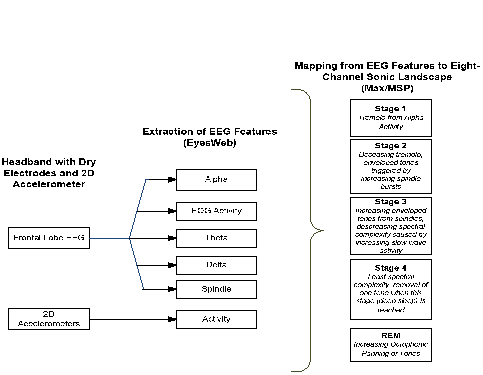
\includegraphics[width=\textwidth]{img-3-eps-converted-to-crop.pdf}
\caption{The MS\&WM Architecture:  The components of the process (1) data
acquisition using a headband on each of four performers, (2) the extraction of
the acquired signals into sleep staging features and (3) the mapping to the
octophonic sound environment.}
\label{Ouzounian:fig:2}
\end{figure}

\section{Performance}

\begin{quotation}
Though awake, one remains under the spell of the dream\ldots{} (Walter Benjamin, \textit{One-Way Street} \cite{Benjamin:1979})
\end{quotation}

\textit{MS\&WM }was presented on three occasions in the summer of 2011.  A
preview performance was given on 4--5 June at the Diapason Gallery in Brooklyn, as
part of BioRhythm: Music and the Body series hosted by Science Gallery Dublin for
the World Science Festival.  On 25--26 June, it was premiered at the BEAM Festival
in Uxbridge; this performance was followed with a breakfast Q\&A with audiences.
A third performance, which was also followed by a Q\&A session with audiences,
took place at Green Man Festival in Wales on 20--21 August.

On all three occasions, the four performers were volunteers---friends,
colleagues, and strangers who offered the use of their brainwaves for a night.
The performances took place in very different settings: an intimate sound art
gallery with a large picture window overlooking the Brooklyn Bridge, where
visitors could sit on chairs and sofas, or sleep on carpeted floors; a large,
darkened auditorium where about forty mattresses were laid out for audiences and
participants; and a large tent in an outdoor festival, where most audiences were
prepared to camp for the weekend. On each occasion audiences were invited to
bring what they needed to ensure comfortable sleep if they were planning to stay
for the duration.

Due to the particular exigencies of the work, the preview performance at the
Diapason Gallery was the first time the authors were privy to how \textit{MS\&WM
}might work outside the studio setting.  We had undertaken different tests in the
studio to learn how different kinds of brainwave activity might result in
different kinds of sound, and had recorded data relating to individuals'
brainwaves during different stages of the Sleep-Wakefulness Cycle (SWC) in order
to test this in studio. Still, the particular dynamics of an 8-hour performance
featuring four performers (all with unique, unpredictable sleep patterns)
remained unknown until the time of performance.

In each of the performances, we had both `light' and  `heavy' sleepers. The
light sleepers woke quite often throughout the night and very rarely encountered
deep sleep.  This caused the presence of frequent tremolo activity from fading in
and out of drowsiness (stage 1) sleep.  Frequent, rapid spindles from stage 2
sleep were also prominent.  Since `light' sleepers never reached stage 4 sleep,
their four tones were always complex and no tones were removed from their initial
allotment of four.  On the other hand, the `deep' sleepers almost never woke up
and reached stage four sleep several times throughout the night.  Thus, they
created an almost perfect counterpoint to the `light' sleepers.  Frequent REM
activity caused the sound to cycle from speaker to speaker.  By being frequently
in stage 3 sleep, they caused long slow spindles to appear.  With the slow-wave
activity, the timbre of their tones were simplified and, by the end of the
evening, they were left with only one note from their original four---sonically
revealing the restful night they experienced.

Notably, the authors (who monitored the sleepers' brainwave activity throughout
the different performances) observed that members of the ensemble perceptibly
responded to changes in the sound environment within the different stages of the
Sleep-Wakefulness Cycle. In the context of this work, such a response can perhaps
be posited as a kind of communication or exchange between the members of the
ensemble, and between the ensemble and its environment.  We also observed that,
within the larger context of the continuous sound environment, sudden or vivid
changes (for example, an unexpectedly loud spindle event) did not typically
awaken the sleepers, although some reported a sense of being continuously pulled
into and out of sleep throughout the night, i.e. kept in a liminal state between
sleep and awakening through changes in the sound environment.

Audiences reported a multitude of different experiences that ranged from intense
to restful to blissful to oblivious. Many reported vivid, imagistic dreams. 
Several commented that, despite being immersed in the sound environment
continuously for many hours, following the performance they had little
recollection of `what it sounded like.'  Others commented on the uniqueness of
the collective sleep experience and of experiencing sound and music in their
sleep. One listener/participant, a composer of electronic music, described her
experience thus:

`It was soothing music, semi-monotonous but continually evolving, with enough
elements particularly when spatialized to generate a need for conscious or
subconscious attention. If concentrating, one could get a sense of a feedback
loop, with the sound correlating with physical state; but this sensation was
rather alien since the correlation was not with bodily change of position or
anything apparent; rather the sound patterns were coincident with changing states
of brain activity of which most of us are not typically aware. For me there was
some sense of relation, i.e. even deliberate control of/generation of sounds. It
was a bit Borg-like since the interconnected sonified mental web of the
collective lying on the floor was externalized, or embodied, as a unified sound
composition in the entire room. I suspect that the composed nature of the
structure, and the specific sounds [that were] selected fostered this sensation.'

In the Q\&A sessions and conversations that followed different performances,
listeners were particularly curious as to how different aspects of the SWC were
articulated in sound, and whether or not things like nightmares could be
discerned in the sound environment. Performers wanted to know more about their
particular sleep patterns and whether they had `performed well' (since the
composition was designed to accommodate any kind of sleep pattern, there was no
`better' or `worse' performance on the part of the performers themselves).

In future performances we plan to experiment with different audio/video DSP
functions and compositional structures in the work, which is in a sense a `model'
or framework than a strictly determined composition. The performance at NIME 2012
will be the first to feature visual projections; we are also planning to develop
an immersive installation model in collaboration with the artist Kate Genevieve,
which will explore aspects of the audience's collective sleep experience.

\section{Conclusion}

In her essay `The Muse is Within: The Psyche in the Century of Science,' Lynn Gamwell predicts that `artists of the next century will be inspired by an awesome new concept of dreamwork that fully integrates neurology with the subjective experience of the self' \cite[p.55]{Gamwell:2000}. \textit{MS\&WM }is an attempt, still in its early stages, at putting neurophysiological science to the service of music and image that are born of, and that give form to, the dream, the process of dreaming, and to dreamers. When Sigmund Freud introduced the concept of the dreamwork as the process whereby the mind produces the manifest dream \cite{Freud:1927}, his theory inspired not only psychoanalytic communities, but myriad artistic communities as well (see \cite[p.9]{Ruhs:2000}).

In Ouzounian and Griffin's overnight work \textit{EDEN EDEN EDEN}, the
continuously evolving patterns of sound and image were conceived as a `memory
processing ritual.' The programme notes read:

`Aural and visual acts become chaotically resonant through their continual
repetition. Members of the audience, who are invited to sleep during the
performance, shift between waking and dreaming states. Afterwards, their memories
coincide.' (Ouzounian and Griffin 2009) \cite{Ouzounian:2009}

\textit{EDEN EDEN EDEN }proposed that the collective experience of continuous,
repetitive, and continuously evolving patterns of sound and image within
different states of consciousness could enable co-incidental `resonant' memories
to emerge. \textit{Music for Sleeping \& Waking Minds} proposes that
communication (understood in its broadest sense, as the exchange of thought) can
occur simultaneously within and between multiple states of consciousness, and
that an intelligent, shared consciousness can emerge from this communication. 
Although this idea is still in its nascent stages and is shaped through an
entirely experimental approach, it encourages a new understanding of the
dreamwork as a shared experience, and of the creation of music as viewed through
the lens of a collective dream.

\begin{acknowledgement}
The authors wish to thank all those friends and colleagues who have presented, participated in, and supported \textit{MS\&WM}.
\end{acknowledgement}

\section*{Author Commentary: New Musical Intimacies}

\paragraph{Gascia Ouzounian, R. Benjamin Knapp, Eric Lyon}

\textbf{Ouzounian:} \textit{Music for Sleeping \& Waking Minds} (2010-12) was the second in a series of overnight works---or, more precisely, music for sleeping audiences---that I have been developing in collaboration with different artists, musicians and engineers since 2009. The first, \textit{EDEN EDEN EDEN} (2009), was created with the filmmaker Chlo\'e Griffin, and entailed a continuously evolving, six-and-a-half-hour composition for string ensemble and film. It was performed overnight, starting around midnight, and audiences could experience the work while awake and while asleep.

\textit{Music for Sleeping \& Waking Minds }emerged from my ongoing collaboration with the Biomuse Trio, an ensemble that explores the use of physiological sensors in the context of musical performance and composition. \cite{Lyon:2014,Ouzounian:2012} It involved four sleeping performers who, while wearing head-mounted EEG sensors, generate an audiovisual environment composed of 8-channel sound and visual projections that correspond to sleep staging. Again, audiences were invited to spend the night, and could experience this work in multiple states of attention, including sleeping and dreaming. However, in this instance, the performers' only task was to fall asleep and awaken as they normally would.

More recently, I have collaborated with Christopher Haworth and Julian Stein to create \textit{Long for this World} (2013-15), an interactive, software-based work that allows listeners to create their own music for sleeping \cite{Ouzounian:2013}. \textit{Long for this World} was substantially different from the other compositions in that listeners could experience it at their leisure, in the comfort of their own homes, and could determine, to a much larger degree, the musical content of the work.

These compositions for sleeping audiences are intended to pose questions that bear much further reflection, and to cultivate musical experiences that we may not normally encounter in either concert listening or in listening to recorded music. How do we experience sound in different states of attention, like sleeping and awakening, and how do these experiences affect us differently? How do we communicate with one another, as performers, if we are not fully conscious? What do these communications tell us about ourselves, and about what we conceive communication to be, or, for that matter, what we believe music to be? How do we experience our environment, including our immediate aural and social environments, within collective modes of sleeping? If we create our own music for sleeping, what is it that we want this music to `do' for us, and how can we translate these motivations into musical ideas? Must concert listening always involve focused or attentive listening, the kind of listening that music theory presumes, or is that kind of listening simply a route towards analysis? How would music be different if it was composed for everyday life activities like sleeping, and not necessarily as `an accompaniment' to those activities, but as an integral part of those activities themselves?

\textbf{Knapp:} The limited notion of the DMI was challenged in this work. Since this paper, a more abstract relation between physical state and sound is now accepted as a complement to the notion of the precise physiological DMI. State of consciousness, emotional state, and physical position can all be incorporated in the relationship between performer and music.

\textbf{Lyon:} It seems to me that there is a special aspect of intimacy to \textit{Music for Sleeping \& Waking Minds}. On the surface, the sleepers' performance is involuntary in its particulars. They simply relax and go to sleep; the active musical construction of the octophonic sound that the audience hears is created by a combination of head-mounted sensors, brainwave pattern recognition, and spatial sonification algorithms. And yet the method of data capture from brainwaves provides a sense of intimacy, as if the listener is inside an overlapping dreamscape constructed by four people who have withdrawn from the direct experience of reality. This special sense of performance intimacy seems to me a unique attribute of this composition.

In a more recent piece by two of the authors, a different but powerful form of performance intimacy was observed. \textit{Dualities}, composed by Eric Lyon, is scored for cello, Biomuse, and ensemble. The piece was premiered by the Crash Ensemble at Virginia Tech in 2015, with Kate Ellis on cello, and Ben Knapp performing Biomuse. Although the two soloists were spatially separated on stage, their performance interactions were understood by several audience members to be tightly integrated and intimate, with a profound level of musical communication. These two examples suggest that in NIME-based performances, an audience's perception of intimacy is a key element to a successful performance.

\section*{Expert Commentary: To Sleep, Perchance To Dream}

\paragraph{Sile O'Modhrain}

In \textit{Music for Sleeping and Waking Minds}, Ouzounian et al present us with  a consummate example of a novel interaction paradigm for the realization of musical intent.  The intent is to create a shared space of experience, at once intimate and vulnerable, where performers simply fall asleep in the company of an audience.  Patterns arising from the cyclical brain-wave activity of the sleepers are used as control signals for both visual and musical elements of the work.  Musically, the piece is comprised of octaphonic drones whose pitches are allocated across the distributed array of sensors so that changes in the activity of individual performer's brainwaves subtly affect the progression of the music while not disturbing the drone-like quality of the evolving sound.  The drone, in turn, lulls the audience toward sleep so that they, too, are drawn into this intimate vulnerable space.  

For over 30 years, Ben Knapp, in conjunction with other collaborators,  has worked to design body-worn sensing systems for capturing biometric signals. He has also played a pivotal role in defining a new field around the concept of biocontrol for musical applications.  In Biomuse \cite{Knapp:1990}, he brought to the community the first robust platform for tracking heartrate, galvanic skin response and brainwave activity that could be used in a real-time performance environment for the control of sound. In 2008, he joined forces with Eric Lyon and Gascia Ouzounian to form the Biomuse Trio.  The trio has developed a performance practice that integrates traditional classical performance, laptop processing of sound and the transduction of bio-signals for the control of musical gesture.  The work of the ensemble encompasses hardware design, audio signal processing, bio-signal processing, composition, improvisation and gesture choreography \cite{Ortiz:2012}.  In 2005, Knapp and Cook introduced the concept of Integral Music Control, a technique for assessing the composite gestures and emotional state of a group of performers, audience members, or both \cite{Knapp:2005}. Knapp says: 

\begin{quotation}
When I first started doing this research, I was interested in exploring the language of physiological and emotional interface design for musical, artistic or therapeutic applications. My first questions were about the tensions between sonification and musicalization. \ldots With the concept of the integral music controller and my more recent work in mobile environments, I am more specifically interested in the larger picture questions of emotional connection and empathy \cite{Ouzounian:2012}.
\end{quotation}

Beyond its integrity as a composition, the contributions of \textit{Music for Sleeping and Waking Minds}  are both the technical infrastructure that makes the work possible, and the questions that it raises about the shared role that performers and audiences play in creating musical experience.  ``When I conceived the composition,'' Ouzounian said 

\begin{quotation}
I was actually thinking about it as a kind of ensemble communication between the performers, but in different states of attention and consciousness. \cite{Ouzounian:2015} 
\end{quotation}

In drawing upon the evolving patterns of sleep, the authors create this space for shared subconscious experience.  In doing so, they provide a compelling demonstration of the potential for Knapp and Cook's technique for Integral Musical Control \cite{Knapp:2005}.  More importantly, this piece provides a timely compositional critique of the all-too-familiar focus on ``interface'' as the means of communicating conscious performative intent.  

